\chapter{Evaluering af Metoder}\label{ch:evalmet}
I dette kapitel vil vi evaluere Affect Grid og 3E metoderne. Her kigger vi nærmere på den opsamlede data, og giver udtryk for vores egen oplevelse af metoderne. Ifølge Woolrych i \cite{Woolrych} er det vigtigt at forstå en metode som en mængde af konfigurerbare resourcer. Ofte er en metode blot en vag opskrift, der giver os en eller flere resourcer at arbejde med. For både Affect Grid og 3E er vi kun blevet stillet med en måde, hvorpå vi kan indsamle data. Vi har selv besluttet, hvordan opgaver udvælges, hvordan data analyseres osv. På baggrund af dette kan vi ikke lave en endelig dom over metoderne. Vi kan dog beskrive, hvordan vi mener de forskellige resourcer burde udvælges og konfigureres.

\section{Affect Grid}\label{sec:evalAG}
Med 11 markeringer fra alle 4 personer endte Affect Grid med at indsamle 44 datapunkter. På \cref{tab:AG} har vi forsøgt at analysere dette datasæt med nogle standard statistiske metrikker. Vi ser at brugere i gennemsnit følte sig neurale ift. både fornøjelse og ophidelse. Dog er der en høj standardafvigelse, hvilket kræver dybere undersøgelse.  

\begin{table}[]
\centering
\caption{Statistiske metrikker over Affect Grid data}
\label{tab:AG}
\begin{tabular}{|l|l|c|}
\hline
                  & Fornøjelse & Ophidelses               \\ \hline
Antal             & 44         & 44                       \\ \hline
Gennemsnit        & 5.3        & 5.7                      \\ \hline
Standardafvigelse & 2.0        & 2.2                      \\ \hline
Min               & 1.0        & \multicolumn{1}{l|}{1.0} \\ \hline
Max               & 1.0        & \multicolumn{1}{l|}{1.0} \\ \hline
\end{tabular}
\end{table}

På \cref{fig:hexbin} har vi plottet dataen på et hexbin diagram. Dette viser udspredelse i langt større grad. Selvom vi ser at mange punkter er placeret neutralt omkring midten, så bliver alle hjørner af diagrammet berørt. Ved at kigge nærmere på hvordan brugere har markeret, ser vi også en stor forskel i, hvordan enkelte opgaver opleves. Dette kan ses i \cref{app:AG}, hvor et søjlediagram over markeringerne er lavet for hver bruger. Generelt ser vi dog nogle større negative udsving, når brugerne er færdige med opgaver som de har haft problemer med. Brugerne bliver da ikke nødvendigvis stimulerede af at overkomme en svær udfordring. 

\begin{figure}[h]
\centering
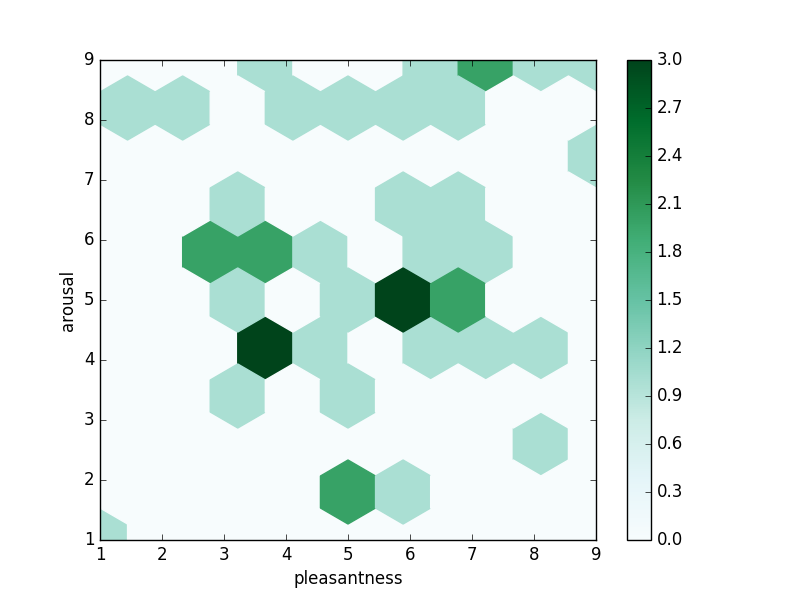
\includegraphics[width=0.6\textwidth]{hexbin.png}
\caption{Hexbin diagram over Affect Grid data}
\label{fig:hexbin}
\end{figure}

Samlet set viser dataen at brugerne har oplevet interaktionen med Codecademy på meget forskellige måder. Fra at have observeret brugerne under evalueringen regner vi dog ikke med, at forskellen skulle være så stor. To faktorer vi tænker kan have haft en indflydelse på forskellen er; brugeres initielle sindelag samt deres forståelse af metoden.

I \cref{app:AG} observerer vi at det første kryds sat af brugerne afviger meget fra hinanden. Da brugerne endnu ikke har interageret med systemet på dette punkt, regner vi ellers med at de markerer i samme område. Dette tyder på at brugerne har haft forskellige mentale udgangspunkter, hvilket har haft en indflydelse på deres oplevelse. Dette gør det svært at sammenligne data fra enkelte brugere. Vi regner dog med at dette problem kunne løses ved at indsamle data fra flere brugere. Dog kunne det være interessant at kigge nærmere på, hvordan data kunne normaliseres ud fra en brugers initielle sindelag.

Det er også muligt at hver bruger har haft en forskellig forståelse af metoden. Bruger 3 er for eksempel mere tilbøjlig til at hoppe ud i ekstremer end bruger 2. Dette kunne tyde på en forskel i hvordan ekstremer opfattes. Vi observerede også desiderede forståelsesproblemer, hvor en bruger spurgte ind til modellen under evaluering. Det lader altså til, at vi skulle have anvendt en anden teknik til at forklare modellen. En ad hoc forklaring, som vi gav, giver ikke nok forståelse. 

Affect Grid blev originalt valgt, da den kunne bruges til at indsamle data under evaluering, uden at trække brugeren ud af interaktionen. Vi finder dog at brugerne stadigvæk brugte meget tid på at overveje, hvor deres krydser skulle sættes. Dette kan relatere sig til forståelseproblemer som nævnt overfor. Det er problematisk, da brugerne bliver trukket ud af interaktionen. Brugerne endte muligvis også med at skulle markere for ofte. Der skal være en balance, hvor vi får nok data uden at brugeren forstyres. 

Alt i alt ser vi et potentialle i Affect Grid. Dog kræver metoden en større indsats fra vores side for få brugerne til at forstå den. Dette med henblik på at de de får den samme opfattelse og hurtigere kan markere på grid'et. Samtidig må der kræves en mere struktureret teknik til at finde ud af, hvornår der skal markeres under evaluering.  


\section{3E}\label{sec:eval3E}